%furtherGraphs
%Hier weitere Graphen hinzuf�gen, die nicht so wirklich in den Hauptteil geh�ren, aber trotzdem erw�hnt werden sollten

\begin{figure}[h]
	\centering
		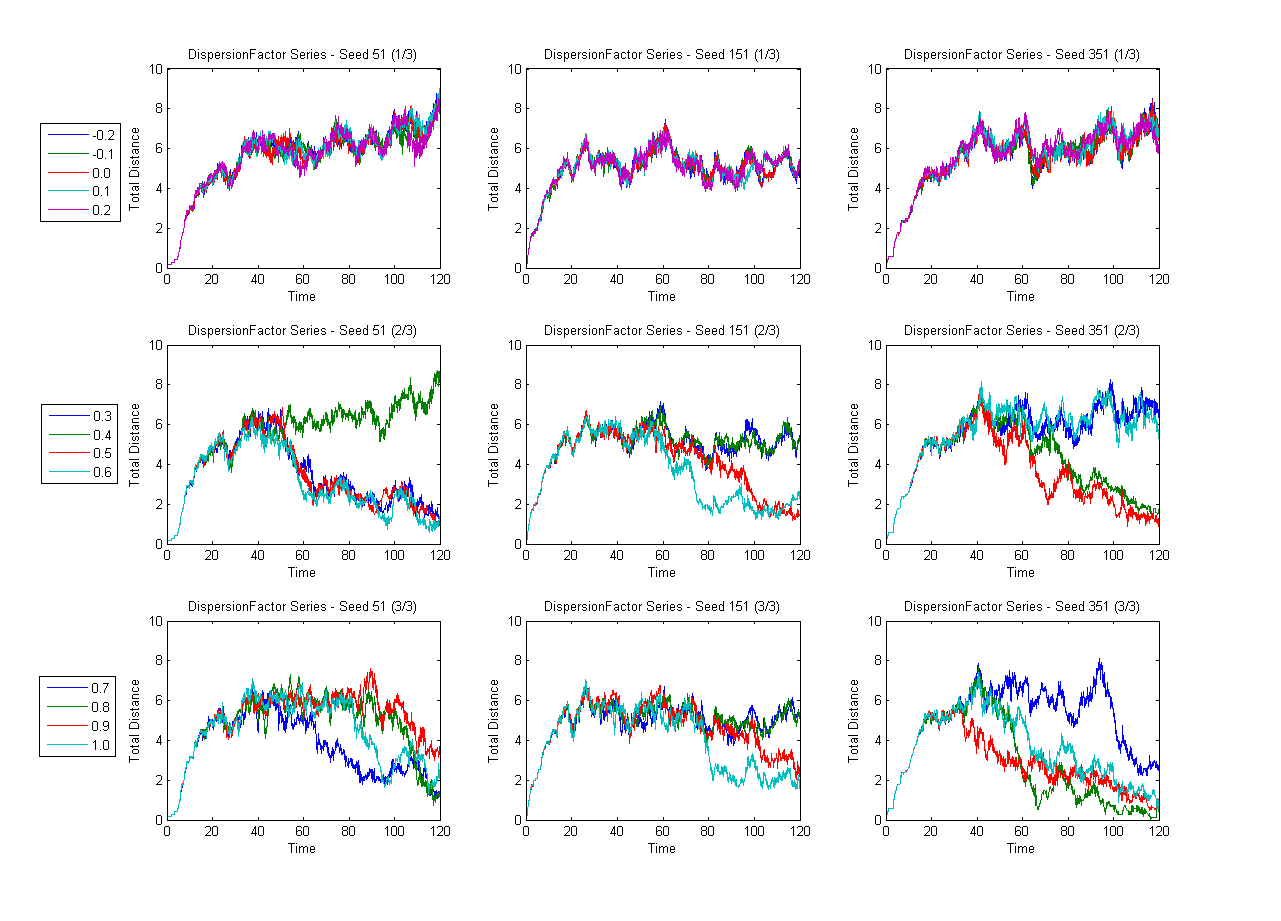
\includegraphics[width=1.00\textwidth]{pictures/ADistanceSeedsFactors.png}
	\caption{Another representation of figure \ref{fig:AAllInOne}, split up into a $3\times 3$ composition for a better view on the single lines.}
	\label{fig:ADistanceSeedsFactors}
\end{figure}

\begin{figure}[h!]
	\centering
		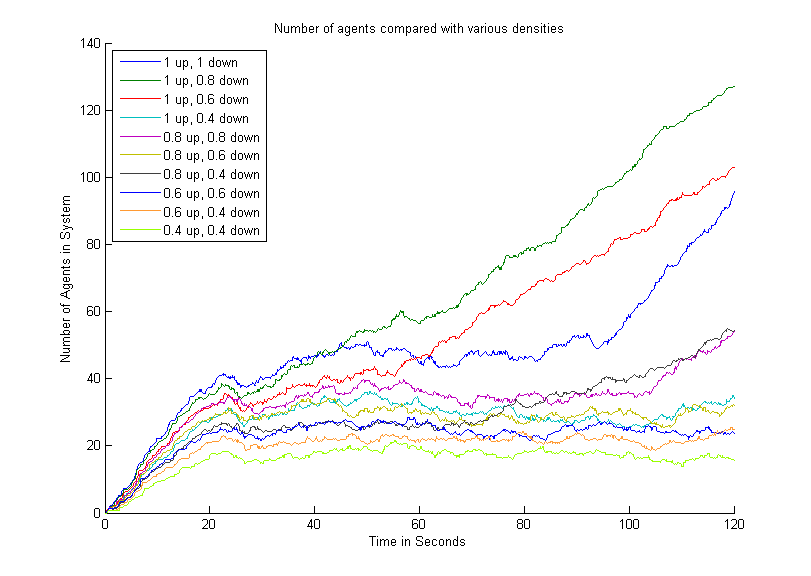
\includegraphics[width=1.0\textwidth]{pictures/AAllAveragesInOnePlot.png}
	\caption{Another representation of figure \ref{fig:AAllAveragesScaled}, where the number of agents is not scaled. It shows the total number of agents in the system for various combinations of flux densities with respect to time. The used flux densities are given in the graph legend. As soon as the total number of agents increases strongly, a jam has formed. The mean over three simulations with different seeds was taken for each case. As expected, high flux densities caused massive jams.}
	\label{fig:AAllAveragesInOnePlot}
\end{figure}
